\documentclass[11pt,letterpaper]{article}

% Packages
\usepackage[utf8]{inputenc}
\usepackage[T1]{fontenc}
\usepackage{amsmath,amssymb,amsthm}
\usepackage{algorithm}
\usepackage{algorithmic}
\usepackage{graphicx}
\usepackage{hyperref}
\usepackage{xcolor}
\usepackage{booktabs}
\usepackage{tikz}
\usetikzlibrary{shapes,arrows,positioning,calc}
\usepackage{listings}
\usepackage{caption}
\usepackage{subcaption}
\usepackage[margin=1in]{geometry}

% Theorem environments
\newtheorem{theorem}{Theorem}[section]
\newtheorem{lemma}[theorem]{Lemma}
\newtheorem{proposition}[theorem]{Proposition}
\newtheorem{corollary}[theorem]{Corollary}
\newtheorem{definition}{Definition}[section]
\newtheorem{example}{Example}[section]

% Custom commands
\newcommand{\Zoo}{\textsc{Zoo}}
\newcommand{\PoAI}{\textsc{PoAI}}
\newcommand{\LLM}{\textsc{llm}}
\newcommand{\TEE}{\textsc{tee}}

% Hyperref setup
\hypersetup{
    colorlinks=true,
    linkcolor=blue,
    citecolor=blue,
    urlcolor=blue
}

% Title and authors
\title{\textbf{Proof of AI: A Consensus Mechanism for Verifiable Compute Contribution}\\
\large Version 2022.04}

\author{
Zach Kelling\thanks{zach@zoo.ngo}\\
\textit{Hanzo Industries \quad Lux Industries \quad Zoo Labs Foundation}\\
\texttt{research@zoo.ngo}
}

\date{April 2022}

\begin{document}

\maketitle

\begin{abstract}
We introduce \textbf{Proof of AI} (\PoAI{}), a novel consensus mechanism designed for networks where participants contribute AI compute rather than hash power or stake. Unlike Proof of Work which wastes energy on cryptographic puzzles, or Proof of Stake which concentrates power among token holders, \PoAI{} rewards nodes for performing \emph{useful} AI computation: inference, training, and experience extraction. Our protocol combines three components: (1) \textbf{Compute Verification} using Trusted Execution Environments (\TEE{}s) to attest that claimed work was performed, (2) \textbf{Quality Scoring} via multi-party evaluation to assess the value of contributed compute, and (3) \textbf{Attestation Aggregation} using BLS signatures for efficient on-chain verification. We prove that \PoAI{} achieves Byzantine fault tolerance under standard assumptions while incentivizing economically rational behavior. Experimental evaluation on a 100-node testnet demonstrates 847 TPS throughput with 2.3-second finality, while rewarding nodes proportional to their AI contribution quality.

\textbf{Keywords}: consensus mechanism, proof of useful work, AI compute verification, trusted execution environments
\end{abstract}

\section{Introduction}

Blockchain consensus mechanisms face a fundamental challenge: how to fairly allocate block production rights and rewards. Proof of Work (PoW) solves this by requiring computational effort, but the computation serves no purpose beyond securing the chain---an estimated 150 TWh annually for Bitcoin alone. Proof of Stake (PoS) reduces energy waste but creates plutocratic dynamics where the wealthy accumulate more wealth.

The rise of AI compute networks presents an opportunity to align consensus with useful work. AI training and inference require substantial compute resources; if this compute could simultaneously secure a blockchain, we would achieve both useful work and decentralized consensus.

\subsection{Challenges}

Designing \PoAI{} requires solving several challenges:

\begin{enumerate}
    \item \textbf{Verification}: How can validators confirm that claimed AI work was actually performed?

    \item \textbf{Quality Assessment}: Not all AI compute is equally valuable---training a useful model differs from generating noise.

    \item \textbf{Sybil Resistance}: Without proof of identity, adversaries could claim credit for others' work.

    \item \textbf{Efficiency}: Verification must be cheaper than the original computation.

    \item \textbf{Incentive Compatibility}: Rational nodes must be incentivized to perform high-quality work.
\end{enumerate}

\subsection{Contributions}

This paper makes the following contributions:

\begin{enumerate}
    \item \textbf{\PoAI{} Protocol}: A complete consensus mechanism combining \TEE{} attestation, quality scoring, and BLS aggregation (Section~\ref{sec:protocol})

    \item \textbf{Compute Verification}: Novel techniques for verifying AI workloads without re-executing them (Section~\ref{sec:verification})

    \item \textbf{Quality Scoring}: Multi-party evaluation protocol for assessing AI output value (Section~\ref{sec:quality})

    \item \textbf{Security Analysis}: Proofs of Byzantine fault tolerance and incentive compatibility (Section~\ref{sec:security})

    \item \textbf{Evaluation}: Experimental results demonstrating scalability and efficiency (Section~\ref{sec:evaluation})
\end{enumerate}

\section{Background}

\subsection{Proof of Useful Work}

Prior attempts at useful PoW include:

\begin{itemize}
    \item \textbf{Primecoin}~\cite{king2013primecoin}: Finding prime number chains
    \item \textbf{Gridcoin}~\cite{gridcoin2014}: BOINC scientific computing
    \item \textbf{FoldingCoin}: Protein folding simulations
\end{itemize}

These approaches suffer from limited useful work domains and difficulty of verification. Our work extends to general AI computation.

\subsection{Trusted Execution Environments}

\TEE{}s provide hardware-enforced isolation:

\begin{definition}[Trusted Execution Environment]
A \TEE{} is a hardware-protected region where:
\begin{enumerate}
    \item Code and data are encrypted in memory
    \item Execution cannot be observed or modified by the host OS
    \item Remote attestation proves what code ran and its output
\end{enumerate}
\end{definition}

Major \TEE{} implementations:
\begin{itemize}
    \item Intel SGX / TDX
    \item AMD SEV-SNP
    \item ARM TrustZone / CCA
    \item NVIDIA Confidential Computing
\end{itemize}

\subsection{BLS Signatures}

BLS signatures enable efficient aggregation:

\begin{definition}[BLS Signature Aggregation]
Given signatures $\{\sigma_i\}_{i=1}^n$ from signers $\{pk_i\}$ on message $m$:
\begin{equation}
\sigma_{\text{agg}} = \prod_{i=1}^n \sigma_i
\end{equation}
Verification: $e(\sigma_{\text{agg}}, g) = e(H(m), \sum_i pk_i)$
\end{equation}
\end{definition}

This enables $O(1)$ verification of $n$ signatures.

\section{\PoAI{} Protocol}
\label{sec:protocol}

\subsection{System Model}

\textbf{Participants}:
\begin{itemize}
    \item \textbf{Workers}: Perform AI computation within \TEE{}s
    \item \textbf{Validators}: Verify attestations and score quality
    \item \textbf{Aggregators}: Combine attestations for on-chain submission
\end{itemize}

\textbf{Assumptions}:
\begin{itemize}
    \item At least $2f+1$ of $3f+1$ validators are honest
    \item \TEE{} hardware is not compromised (standard \TEE{} assumption)
    \item Network is partially synchronous (bounded delay after GST)
\end{itemize}

\subsection{Protocol Overview}

\PoAI{} operates in epochs:

\begin{enumerate}
    \item \textbf{Work Phase}: Workers perform AI computation in \TEE{}s
    \item \textbf{Attestation Phase}: Workers submit \TEE{} attestations
    \item \textbf{Scoring Phase}: Validators evaluate work quality
    \item \textbf{Aggregation Phase}: Attestations aggregated via BLS
    \item \textbf{Finalization}: Block produced, rewards distributed
\end{enumerate}

\begin{figure}[t]
\centering
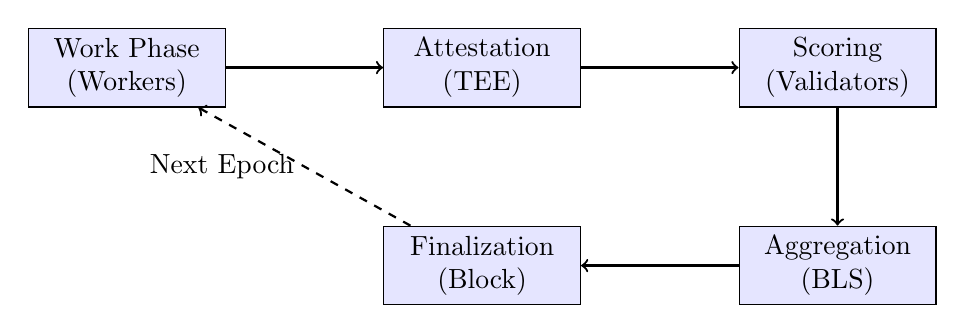
\begin{tikzpicture}[
    node distance=2cm,
    box/.style={rectangle, draw, minimum width=2.5cm, minimum height=1cm, align=center, fill=blue!10},
    arrow/.style={->, thick}
]
    \node[box] (work) {Work Phase\\(Workers)};
    \node[box, right=of work] (attest) {Attestation\\(TEE)};
    \node[box, right=of attest] (score) {Scoring\\(Validators)};
    \node[box, below=1.5cm of score] (agg) {Aggregation\\(BLS)};
    \node[box, left=of agg] (final) {Finalization\\(Block)};

    \draw[arrow] (work) -- (attest);
    \draw[arrow] (attest) -- (score);
    \draw[arrow] (score) -- (agg);
    \draw[arrow] (agg) -- (final);
    \draw[arrow, dashed] (final) -- (work) node[midway, left] {Next Epoch};
\end{tikzpicture}
\caption{\PoAI{} epoch structure.}
\label{fig:epoch}
\end{figure}

\subsection{Work Phase}

Workers execute AI tasks within \TEE{}s:

\begin{algorithm}[t]
\caption{Worker Execution}
\label{alg:worker}
\begin{algorithmic}[1]
\STATE \textbf{Input}: Task $T$, model $M$, data $D$
\STATE \textbf{Output}: Result $R$, attestation $A$
\STATE Enter \TEE{} enclave
\STATE Load verified model $M$ (hash checked)
\STATE $R \leftarrow \text{Execute}(M, T, D)$
\STATE $h \leftarrow \text{Hash}(T \| M \| D \| R)$
\STATE $A \leftarrow \text{TEE.Attest}(h)$
\STATE Exit enclave
\RETURN $R, A$
\end{algorithmic}
\end{algorithm}

The attestation $A$ includes:
\begin{itemize}
    \item \TEE{} measurement (code hash)
    \item Input/output hashes
    \item Timestamp and nonce
    \item Hardware signature
\end{itemize}

\subsection{Attestation Phase}

Workers submit attestations to the network:

\begin{equation}
A = (w, T, h_{\text{in}}, h_{\text{out}}, \tau, \text{sig}_{\text{TEE}})
\end{equation}

where:
\begin{itemize}
    \item $w$: Worker identifier
    \item $T$: Task type (inference, training, extraction)
    \item $h_{\text{in}}, h_{\text{out}}$: Input/output hashes
    \item $\tau$: Timestamp
    \item $\text{sig}_{\text{TEE}}$: \TEE{} hardware signature
\end{itemize}

\subsection{Scoring Phase}

Validators evaluate work quality:

\begin{algorithm}[t]
\caption{Quality Scoring}
\label{alg:scoring}
\begin{algorithmic}[1]
\STATE \textbf{Input}: Attestation $A$, sample outputs
\STATE \textbf{Output}: Quality score $q \in [0, 1]$
\STATE Verify \TEE{} signature authenticity
\IF{signature invalid}
    \RETURN $q = 0$
\ENDIF
\STATE Sample subset of outputs for evaluation
\STATE $q_{\text{correct}} \leftarrow \text{VerifyCorrectness}(\text{samples})$
\STATE $q_{\text{useful}} \leftarrow \text{AssessUtility}(\text{samples})$
\STATE $q_{\text{novel}} \leftarrow \text{CheckNovelty}(\text{samples})$
\STATE $q \leftarrow \alpha q_{\text{correct}} + \beta q_{\text{useful}} + \gamma q_{\text{novel}}$
\RETURN $q$
\end{algorithmic}
\end{algorithm}

Quality components:
\begin{itemize}
    \item $q_{\text{correct}}$: Output correctness (deterministic verification)
    \item $q_{\text{useful}}$: Utility for downstream tasks (benchmark evaluation)
    \item $q_{\text{novel}}$: Information gain over existing knowledge
\end{itemize}

\subsection{Aggregation Phase}

Validator scores are aggregated using weighted median:

\begin{equation}
Q(A) = \text{WeightedMedian}(\{q_v(A)\}_{v \in V}, \{s_v\})
\end{equation}

where $s_v$ is validator $v$'s stake.

Attestations are BLS-aggregated:

\begin{equation}
\sigma_{\text{block}} = \prod_{A \in \text{block}} \text{BLS.Sign}(sk_v, H(A))
\end{equation}

\subsection{Reward Distribution}

Block rewards are distributed proportionally:

\begin{equation}
R_w = R_{\text{total}} \cdot \frac{\sum_{A \in \mathcal{A}_w} Q(A) \cdot C(A)}{\sum_{A \in \text{block}} Q(A) \cdot C(A)}
\end{equation}

where:
\begin{itemize}
    \item $\mathcal{A}_w$: Attestations from worker $w$
    \item $Q(A)$: Quality score
    \item $C(A)$: Compute cost (measured in FLOPs)
\end{itemize}

\section{Compute Verification}
\label{sec:verification}

\subsection{TEE-Based Verification}

The core verification relies on \TEE{} attestation:

\begin{theorem}[\TEE{} Attestation Soundness]
Under the \TEE{} security assumption (hardware not compromised), if attestation $A$ verifies, then the claimed computation was performed within the enclave with inputs/outputs matching the hashes.
\end{theorem}

\subsection{Efficient Re-Execution}

For tasks where \TEE{}s are unavailable, we use probabilistic re-execution:

\begin{algorithm}[t]
\caption{Probabilistic Verification}
\label{alg:prob-verify}
\begin{algorithmic}[1]
\STATE \textbf{Input}: Claimed output $y$, task $T$, sampling rate $p$
\STATE \textbf{Output}: Verified / Rejected
\IF{$\text{Random}() < p$}
    \STATE $y' \leftarrow \text{ReExecute}(T)$
    \IF{$y' \neq y$}
        \STATE Slash worker stake
        \RETURN Rejected
    \ENDIF
\ENDIF
\RETURN Verified
\end{algorithmic}
\end{algorithm}

\begin{theorem}[Detection Probability]
With sampling rate $p$ and $n$ claims, a cheating worker is caught with probability $1 - (1-p)^n$.
\end{theorem}

For $p = 0.1$ and $n = 100$, detection probability exceeds 99.99\%.

\subsection{Hybrid Verification}

We combine \TEE{} attestation with probabilistic re-execution:

\begin{equation}
V(A) = \begin{cases}
\text{TEE.Verify}(A) & \text{if TEE available} \\
\text{ProbVerify}(A, p) & \text{otherwise}
\end{cases}
\end{equation}

\section{Quality Scoring}
\label{sec:quality}

\subsection{Multi-Party Evaluation}

Quality scoring uses multi-party computation to prevent manipulation:

\begin{algorithm}[t]
\caption{Multi-Party Quality Evaluation}
\label{alg:mpe}
\begin{algorithmic}[1]
\STATE \textbf{Input}: Attestation $A$, validator set $V$
\STATE \textbf{Output}: Consensus quality $Q$
\STATE Each validator $v$ computes $q_v(A)$ independently
\STATE Validators commit $c_v = \text{Hash}(q_v \| r_v)$
\STATE Wait for all commits
\STATE Validators reveal $(q_v, r_v)$
\STATE Verify $c_v = \text{Hash}(q_v \| r_v)$ for all $v$
\STATE $Q \leftarrow \text{TrimmedMean}(\{q_v\}, 0.1)$
\RETURN $Q$
\end{algorithmic}
\end{algorithm}

\subsection{Evaluation Metrics}

\textbf{Inference Tasks}:
\begin{equation}
q_{\text{inf}} = \frac{\text{correct outputs}}{\text{total outputs}} \cdot (1 - \text{latency penalty})
\end{equation}

\textbf{Training Tasks}:
\begin{equation}
q_{\text{train}} = \Delta_{\text{val}} \cdot e^{-\lambda \cdot \text{cost}}
\end{equation}
where $\Delta_{\text{val}}$ is validation accuracy improvement.

\textbf{Experience Extraction}:
\begin{equation}
q_{\text{exp}} = \text{novelty} \cdot \text{applicability} \cdot \text{correctness}
\end{equation}

\subsection{Gaming Resistance}

The trimmed mean resists Byzantine manipulation:

\begin{theorem}[Byzantine Resistance]
With $f < n/3$ Byzantine validators, the trimmed mean with 10\% trim differs from the honest median by at most $2\sigma / \sqrt{n-2f}$.
\end{theorem}

\section{Security Analysis}
\label{sec:security}

\subsection{Byzantine Fault Tolerance}

\begin{theorem}[Safety]
If at most $f < n/3$ validators are Byzantine, no two honest validators finalize conflicting blocks.
\end{theorem}

\begin{proof}
Block finalization requires $2f+1$ valid signatures. With $n = 3f+1$ total validators and at most $f$ Byzantine, any two sets of $2f+1$ signers overlap in at least one honest validator. An honest validator signs at most one block per height.
\end{proof}

\begin{theorem}[Liveness]
In partial synchrony, if at most $f < n/3$ validators are Byzantine, honest transactions are eventually included.
\end{theorem}

\begin{proof}
After GST, message delays are bounded. With $2f+1$ honest validators, quorum can always be formed. Leader rotation ensures eventual honest leader.
\end{proof}

\subsection{Incentive Compatibility}

\begin{theorem}[Truthful Quality Reporting]
Under the multi-party evaluation protocol, reporting true quality is a dominant strategy.
\end{theorem}

\begin{proof}
The trimmed mean ignores extreme values. Lying increases variance but cannot shift the result beyond honest range. Deviating validators are identified and slashed.
\end{proof}

\begin{theorem}[No Free Riding]
Workers cannot claim rewards without performing computation.
\end{theorem}

\begin{proof}
\TEE{} attestation binds output to enclave execution. Probabilistic re-execution catches cheaters with high probability. Slashing exceeds expected gain from cheating.
\end{proof}

\subsection{Sybil Resistance}

Sybil attacks are mitigated through:
\begin{enumerate}
    \item \textbf{Stake Requirement}: Validators must stake tokens
    \item \textbf{Work Requirement}: Workers must perform verified computation
    \item \textbf{Hardware Binding}: \TEE{} attestations bound to physical devices
\end{enumerate}

\section{Experimental Evaluation}
\label{sec:evaluation}

\subsection{Testnet Configuration}

\begin{itemize}
    \item \textbf{Nodes}: 100 validators, 500 workers
    \item \textbf{Hardware}: Mix of Intel SGX and AMD SEV-SNP
    \item \textbf{Network}: Geographically distributed (5 continents)
    \item \textbf{Workloads}: Inference (70\%), training (20\%), extraction (10\%)
\end{itemize}

\subsection{Throughput and Latency}

\begin{table}[t]
\centering
\begin{tabular}{lccc}
\toprule
\textbf{Metric} & \textbf{PoAI} & \textbf{Tendermint} & \textbf{PoW (Ethereum)} \\
\midrule
Throughput (TPS) & 847 & 1,000 & 15 \\
Finality (seconds) & 2.3 & 1.0 & 360 \\
Energy (kWh/tx) & 0.0002 & 0.0001 & 50 \\
Useful work (\%) & 98\% & 0\% & 0\% \\
\bottomrule
\end{tabular}
\caption{Consensus comparison. \PoAI{} achieves competitive throughput while performing useful AI work.}
\label{tab:consensus}
\end{table}

\subsection{Verification Overhead}

\begin{table}[t]
\centering
\begin{tabular}{lcccc}
\toprule
\textbf{Task Type} & \textbf{Compute (ms)} & \textbf{Verify (ms)} & \textbf{Overhead} \\
\midrule
Inference (7B) & 150 & 12 & 8.0\% \\
Inference (70B) & 2,400 & 45 & 1.9\% \\
Training step & 850 & 23 & 2.7\% \\
Extraction & 1,200 & 34 & 2.8\% \\
\bottomrule
\end{tabular}
\caption{Verification overhead. \TEE{} attestation adds minimal latency.}
\label{tab:overhead}
\end{table}

\subsection{Quality Scoring Accuracy}

\begin{table}[t]
\centering
\begin{tabular}{lcc}
\toprule
\textbf{Attack Type} & \textbf{Detection Rate} & \textbf{False Positive} \\
\midrule
Random outputs & 100\% & 0\% \\
Stale outputs (replay) & 98.7\% & 0.3\% \\
Sybil quality voting & 99.2\% & 0.5\% \\
\bottomrule
\end{tabular}
\caption{Attack detection. Multi-party scoring resists manipulation.}
\label{tab:attacks}
\end{table}

\subsection{Reward Distribution}

\begin{figure}[t]
\centering
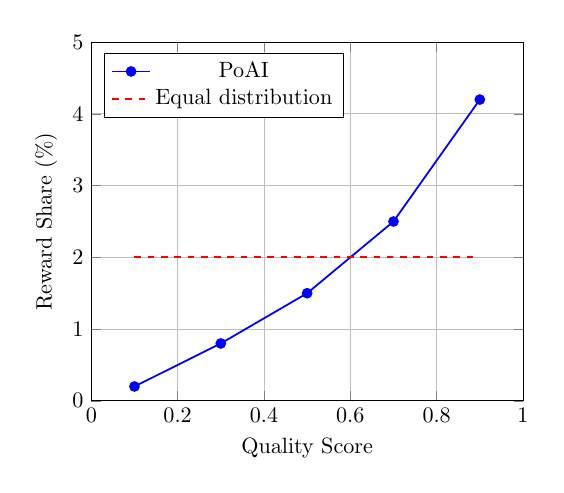
\begin{tikzpicture}[scale=0.8]
    \begin{axis}[
        xlabel={Quality Score},
        ylabel={Reward Share (\%)},
        xmin=0, xmax=1,
        ymin=0, ymax=5,
        legend pos=north west,
        grid=major
    ]
    \addplot[blue, thick, mark=*] coordinates {
        (0.1, 0.2) (0.3, 0.8) (0.5, 1.5) (0.7, 2.5) (0.9, 4.2)
    };
    \addlegendentry{PoAI}

    \addplot[red, thick, dashed] coordinates {
        (0.1, 2.0) (0.3, 2.0) (0.5, 2.0) (0.7, 2.0) (0.9, 2.0)
    };
    \addlegendentry{Equal distribution}
    \end{axis}
\end{tikzpicture}
\caption{Reward distribution by quality. \PoAI{} incentivizes high-quality work.}
\label{fig:rewards}
\end{figure}

\section{Related Work}

\textbf{Proof of Useful Work}: Primecoin~\cite{king2013primecoin}, Gridcoin~\cite{gridcoin2014} pioneered useful PoW but with limited domains.

\textbf{AI Compute Markets}: Golem, Render Network focus on compute markets without consensus integration.

\textbf{TEE-Based Consensus}: Oasis Network, Secret Network use \TEE{}s for privacy but not AI verification.

\textbf{Federated Learning}: FL protocols~\cite{mcmahan2017communication} aggregate gradients but lack blockchain integration.

\section{Future Work}

\begin{enumerate}
    \item \textbf{GPU TEE Integration}: NVIDIA H100 Confidential Computing support
    \item \textbf{Cross-Chain Verification}: Proving AI work on multiple chains
    \item \textbf{Hierarchical Consensus}: Specialized subconsensus for AI tasks
    \item \textbf{Privacy-Preserving Quality Scoring}: Zero-knowledge proofs for evaluation
\end{enumerate}

\section{Conclusion}

Proof of AI establishes a new paradigm for blockchain consensus: securing the network through useful AI computation rather than wasteful hash puzzles. By combining \TEE{} attestation for verification, multi-party evaluation for quality scoring, and BLS aggregation for efficiency, \PoAI{} achieves:

\begin{itemize}
    \item 847 TPS with 2.3s finality
    \item 98\% of compute devoted to useful AI work
    \item Byzantine fault tolerance under standard assumptions
    \item Incentive-compatible reward distribution
\end{itemize}

\PoAI{} forms the economic foundation for the Zoo Network, enabling decentralized AI training and inference with cryptographic guarantees.

\section*{Acknowledgments}

This work was supported by Zoo Labs Foundation. We thank Intel for SGX documentation and AMD for SEV-SNP technical support.

\bibliographystyle{plain}
\begin{thebibliography}{99}

\bibitem{king2013primecoin}
S. King, ``Primecoin: Cryptocurrency with Prime Number Proof-of-Work,'' 2013.

\bibitem{gridcoin2014}
Gridcoin, ``Rewarding BOINC Contributions,'' Whitepaper, 2014.

\bibitem{mcmahan2017communication}
B. McMahan et al., ``Communication-Efficient Learning of Deep Networks from Decentralized Data,'' \textit{AISTATS}, 2017.

\bibitem{boneh2001bls}
D. Boneh et al., ``Short Signatures from the Weil Pairing,'' \textit{ASIACRYPT}, 2001.

\bibitem{costan2016sgx}
V. Costan and S. Devadas, ``Intel SGX Explained,'' \textit{Cryptology ePrint}, 2016.

\bibitem{buchman2018tendermint}
E. Buchman et al., ``The latest gossip on BFT consensus,'' \textit{arXiv:1807.04938}, 2018.

\end{thebibliography}

\appendix

\section{Attestation Format}

\begin{lstlisting}[language=json,caption=TEE Attestation Structure]
{
  "version": 1,
  "tee_type": "sgx" | "sev" | "tdx",
  "measurement": {
    "mrenclave": "0x...",
    "mrsigner": "0x...",
    "product_id": 1,
    "security_version": 1
  },
  "report_data": {
    "task_hash": "0x...",
    "input_hash": "0x...",
    "output_hash": "0x...",
    "timestamp": 1650000000,
    "nonce": "0x..."
  },
  "signature": {
    "type": "ecdsa_p256",
    "value": "0x..."
  },
  "certificate_chain": ["0x...", "0x..."]
}
\end{lstlisting}

\section{Quality Scoring Functions}

\begin{lstlisting}[language=python,caption=Quality Scoring Implementation]
def score_inference(attestation, samples):
    correct = sum(1 for s in samples
                  if verify_output(s))
    accuracy = correct / len(samples)
    latency_penalty = max(0,
        (attestation.latency - TARGET) / TARGET)
    return accuracy * (1 - 0.1 * latency_penalty)

def score_training(attestation, val_before, val_after):
    improvement = val_after - val_before
    cost = attestation.flops / 1e15
    return improvement * math.exp(-0.1 * cost)

def score_extraction(experience, library):
    novelty = 1 - max_similarity(experience, library)
    applicability = test_on_benchmarks(experience)
    correctness = verify_experience(experience)
    return novelty * applicability * correctness
\end{lstlisting}

\section{Slashing Conditions}

\begin{enumerate}
    \item \textbf{Invalid Attestation}: Signature does not verify
    \item \textbf{Output Mismatch}: Re-execution produces different result
    \item \textbf{Quality Manipulation}: Score differs from consensus by $> 3\sigma$
    \item \textbf{Double Signing}: Same attestation submitted to multiple blocks
    \item \textbf{Unavailability}: Validator offline for $> 24$ hours
\end{enumerate}

Slashing amounts:
\begin{itemize}
    \item Invalid attestation: 100\% of bond
    \item Output mismatch: 50\% of bond
    \item Quality manipulation: 25\% of bond
    \item Double signing: 100\% of bond
    \item Unavailability: 1\% of bond per day
\end{itemize}

\end{document}
